\documentclass[11pt,a4paper]{article}

% ── Encoding & fonts ──────────────────────────────────────────────
\usepackage[utf8]{inputenc} \usepackage[T1]{fontenc} \usepackage{lmodern} \usepackage{microtype}

% ── Math ──────────────────────────────────────────────────────────
\usepackage{amsmath,amssymb,amsthm}

% ── Geometry ──────────────────────────────────────────────────────
\usepackage[margin=2.5cm,headsep=10pt]{geometry}
\usepackage{float}

% ── Colour & code ─────────────────────────────────────────────────
\usepackage{xcolor} \usepackage{listings} \lstset{ basicstyle=\ttfamily\small, breaklines=true, frame=single, backgroundcolor=\color{gray!5}, }

% ── Tables ────────────────────────────────────────────────────────
\usepackage{booktabs} \usepackage{tabularx} \usepackage{array}

% ── Graphics ──────────────────────────────────────────────────────
\usepackage{graphicx} \usepackage{caption} \usepackage{subcaption}

% ── Hyperlinks ────────────────────────────────────────────────────
\usepackage[colorlinks=true,linkcolor=blue,citecolor=blue,urlcolor=blue]{hyperref}

% ── Header / footer ───────────────────────────────────────────────
\usepackage{fancyhdr} \setlength{\headheight}{14pt} \pagestyle{fancy} \lhead{Computational Astrophysics --- Project 2} \rhead{\thepage} \cfoot{}

% ── Title ─────────────────────────────────────────────────────────
\title{\textbf{Project 2: MHD Shock-Cloud Interaction}\\[4pt] \large Simulation and Analysis with PLUTO and Independent Python Solvers} \author{Martina García Mejía\\ \small\textit{Computational Astrophysics}\\[4pt] \small June 2026} \date{}

\begin{document}
\maketitle \thispagestyle{fancy}

% ==================================================================
\section{General Description}
% ==================================================================

This project reproduces and analyses the \textbf{2.5D MHD shock--cloud interaction} benchmark from PLUTO's \texttt{Test\_Problems/MHD/Shock\_Cloud/}: a planar magnetised shock strikes an overdense, magnetised spherical cloud and the subsequent evolution exhibits the canonical MHD phenomenology of shocked inhomogeneous media. This is the Dai \& Woodward (1994) setup \cite{dai1994}; the parameter values (post-/pre-shock states, cloud location and radius, embedded oblique magnetic field) are reproduced exactly in our \texttt{inputs/init.c}.
\\

We extended the deliverable spec's ``one example setup'' by running four PLUTO methods: three one-knob variants (setups 01, 02, 09) that isolate the time-stepping and entropy-fix axes, plus a compound setup (02+09) that enables both changes. Two independent Python solvers provide the cross-solver reference: a baseline cell-centred Rusanov/MUSCL/RK2 solver and a constrained-transport (CT) upgrade that keeps the same fluid update while changing the magnetic-field evolution.

\subsection{Governing Equations}

The ideal magnetohydrodynamic (MHD) equations describe a non-relativistic, perfectly conducting, inviscid fluid coupled to a magnetic field. In conservative form with an adiabatic equation of state they read

\begin{equation}
\frac{\partial \rho}{\partial t} + \nabla \cdot (\rho \mathbf{v}) = 0,
\label{eq:cont}
\end{equation}

\begin{equation}
\frac{\partial (\rho \mathbf{v})}{\partial t} + \nabla \cdot \left[ \rho \mathbf{v}\mathbf{v} + \left(p + \tfrac{B^2}{2}\right)\mathbf{I} - \mathbf{B}\mathbf{B} \right] = 0,
\label{eq:mom}
\end{equation}

\begin{equation}
\frac{\partial \mathbf{B}}{\partial t} - \nabla \times (\mathbf{v} \times \mathbf{B}) = 0,
\label{eq:ind}
\end{equation}

\begin{equation}
\frac{\partial E}{\partial t} + \nabla \cdot \left[ \left(E + p + \tfrac{B^2}{2}\right)\mathbf{v} - (\mathbf{v} \cdot \mathbf{B})\mathbf{B} \right] = 0,
\label{eq:e}
\end{equation}

\begin{equation}
\nabla \cdot \mathbf{B} = 0, \qquad p = (\gamma - 1)\,\rho\,\varepsilon.
\label{eq:divb}
\end{equation}

Here $\rho$ is mass density, $\mathbf{v}$ the velocity, $\mathbf{B}$ the magnetic field (with the factor $1/\sqrt{4\pi}$ absorbed), $p$ the gas pressure, $E = p/(\gamma-1) + \tfrac{1}{2}\rho v^2 + \tfrac{1}{2}B^2$ the total energy density, $\varepsilon$ the specific internal energy, and $\gamma = 5/3$ the adiabatic index. Equation~(\ref{eq:divb}) is the solenoidal constraint; its preservation at the discrete level is a central challenge for numerical MHD \cite{brackbill1980, toth2000}.

\subsection{Suppositions and Initial Conditions}

The physics rests on four assumptions: (i) the fluid is classical and non-relativistic; (ii) electrical conductivity is infinite, so the field is frozen into the plasma; (iii) explicit resistivity, viscosity, and thermal conduction are negligible; (iv) the equation of state is adiabatic with constant $\gamma$. For the shock--cloud benchmark these are well justified: dynamical time-scales are far shorter than diffusion time-scales, and post-shock temperatures ($\sim 10^{6}$--$10^{7}$~K in the interstellar analogue) make radiative cooling unimportant on the cloud-crushing time when the density contrast $\chi \lesssim 10$ \cite{shin2008}.
\\

The initial conditions follow the canonical Dai \& Woodward (1994) setup \cite{dai1994}. Two uniform regions are separated by a planar discontinuity at $x = 0.6$.
\\

The calculation is 2.5D: PLUTO is configured with two spatial dimensions but three vector components (\texttt{DIMENSIONS = 2}, \texttt{COMPONENTS = 3}). Thus every plotted field is a function of the $x$--$y$ grid only, while the velocity and magnetic field may still contain $z$-components. In differential form this means $\partial/\partial z = 0$, but $v_z$ and $B_z$ are evolved as part of the state vector. This is essential for this benchmark because the imposed oblique field has a non-zero out-of-plane component $B_z$; the summary panels therefore show eight 2D maps: $\rho$, $v_x$, $v_y$, $v_z$, $B_x$, $B_y$, $B_z$, and $p$.

\medskip
\begin{center}
\begin{tabular}{lccc}
\toprule Region & $\rho$ & $\mathbf{v}$ & $p$ \\ \midrule Post-shock ($x < 0.6$) & 3.86859 & $(0,\,0,\,0)$ & 167.345 \\ Pre-shock ($x \ge 0.6$) & 1 & $(-11.2536,\,0,\,0)$ & 1 \\ \midrule Region & $\mathbf{B}$ & & \\ \midrule Post-shock ($x < 0.6$) & $(0,\,+2.1826182,\,-2.1826182)$ & \\ Pre-shock ($x \ge 0.6$) & $(0,\,+0.56418958,\,+0.56418958)$ & \\ \bottomrule
\end{tabular}
\end{center}
\medskip

An overdense spherical cloud is centred at $(0.8,\,0.5)$ with radius $0.15$, density $\rho_{\mathrm{cloud}} = 10$, and pressure in equilibrium with the ambient pre-shock medium ($p = 1$). The magnetic field inside the cloud matches the pre-shock field, and the cloud velocity is initially zero.
\\

The magnetic field geometry is oblique to the shock normal. In the post-shock region the field lies in the $y$-$z$ plane with equal and opposite components giving $B^2 \approx 9.53$; the post-shock plasma is thermally dominated ($\beta_{\rm post} \approx 35$), while the pre-shock ambient is moderately magnetised ($\beta_{\rm pre} \approx 3.1$). As the shock sweeps past the cloud, this tangential field wraps around it, producing a magnetic draping layer that suppresses KHI on the front side while channelling ablation along the flanks \cite{gregori2000, shin2008, dursi2008}. The oblique field also breaks the top--bottom symmetry of the wake.

\subsection{Boundary Conditions and Time Scales}

Boundary conditions are chosen to isolate the interaction from artificial reflections:
\begin{itemize}
  \item \textbf{Left ($x = 0$):} outflow (zero-gradient), allowing post-shock material to leave without reflection.
  \item \textbf{Right ($x = 1$):} userdef BC reset to the pre-shock state (the outflowing pre-shock material matches this state).
  \item \textbf{Top and bottom ($y = 0,\,1$):} outflow (zero-gradient), allowing material to exit the transverse boundaries.
\end{itemize}

A key dynamical time-scale is the cloud-crushing time \cite{klein1994}:

$$
\tau_{\mathrm{cc}} = \frac{\chi^{1/2}\,R_{\mathrm{cloud}}} {v_{\mathrm{post}}}.
$$

For $\chi = 10$, $R = 0.15$, and $v_{\mathrm{post}} \approx 11.25$, we obtain $\tau_{\mathrm{cc}} \approx 0.042$ in code units. The simulation end-time $t_{\mathrm{stop}} = 0.06$ corresponds to roughly $1.4\,\tau_{\mathrm{cc}}$, enough to capture the cloud-crushing phase.

\subsection{Reference Frame and Shock Mach Numbers}

The shock is stationary at $x = 0.6$ in the lab frame: the post-shock material is at rest ($\mathbf{v}_{\rm post} = \mathbf{0}$) and the pre-shock material flows leftward at $\mathbf{v}_{\rm pre} = (-11.2536,\,0,\,0)$. The relative flow speed in the pre-shock frame is therefore $v_{\rm flow} = 11.2536$. The pre-shock sound speed is $c_s = \sqrt{\gamma p/\rho} = \sqrt{5/3} \approx 1.29$ and the Alfv\'en speed is $c_A = B / \sqrt{\rho} = \sqrt{0.564^2 + 0.564^2} \approx 0.80$. We quote three Mach numbers (definitions used in the literature, \cite{brio1988}):

\medskip
\begin{center}
\small
\begin{tabular}{lcc}
\toprule Definition & Speed used & Pre-shock Mach number \\ \midrule
Sound Mach (PLUTO log) & $c_s$ & $\mathcal{M}_s \approx 8.7$ \\
Alfvén Mach            & $c_A$ & $\mathcal{M}_A \approx 14$ \\
Fast magnetosonic Mach  & $\sqrt{c_s^2 + c_A^2}$ (B tangential) & $\mathcal{M}_f \approx 7.4$ \\ \bottomrule
\end{tabular}
\end{center}
\medskip

PLUTO's per-step log reports $\mathcal{M} = 8.76$ using the pure sound speed; this is the value quoted throughout the per-setup sections below whenever we say ``the Mach number''.

\subsection{Algorithmic Decisions}

The four PLUTO setups differ in two numerical-scheme axes while keeping all other parameters identical:

\medskip
\begin{center}
\begin{tabular}{lccccr}
\toprule Setup & Time stepping & Reconstruction & $\nabla\!\cdot\!\mathbf{B}$ & Entropy fix & Solver \\ \midrule
01    & RK2                  & LINEAR & CT   & NO         & Roe \\
02    & Characteristic Tr.  & LINEAR & CT   & NO         & Roe \\
09    & RK2                  & LINEAR & CT   & SELECTIVE  & Roe \\
02+09 & Characteristic Tr.  & LINEAR & CT   & SELECTIVE  & Roe \\ \bottomrule
\end{tabular}
\end{center}
\medskip


Setups 01 vs 02 isolate the time-stepping axis; setups 01 vs 09 isolate the entropy-fix axis; setup 02+09 then shows the compound effect when Characteristic Tracing and the SELECTIVE entropy fix are enabled together. 
\\

The remaining Shock\_Cloud setups (03 uses Hancock + 8-wave; 04--08 are 3D, two of them with AMR) are out of scope for this 2D study. All four PLUTO runs share grid $256^2$, $\mathrm{CFL}=0.4$, and identical IC/BC.

\subsubsection{Time stepping: RK2 vs Characteristic Tracing}

The time integrator takes the cell-averaged state at $t^n$ and produces the state at $t^{n+1} = t^n + \Delta t$. For an MHD shock at Mach $\approx 9$ the local Mach number varies sharply across the shock front, so the timestep the CFL condition allows ($\Delta t \propto 1 / \max(|v| + c_f)$) is set by a small number of cells. The two schemes differ in how they march through that step.
\\

\textbf{Runge--Kutta 2 (RK2, Heun's method)} is a strong-stability-preserving (SSP) two-stage explicit integrator: predict the half-step, evaluate the flux, then correct. It is the workhorse of modern MHD codes because it is simple, monotonicity-preserving under CFL$\le 1$, and adds numerical diffusion primarily through the half-step predictor. Its physical cost is a small amount of extra smoothing near strong discontinuities; with our CFL of 0.4 this manifests as slightly broader shock profiles than a higher-order scheme would produce.
\\

\textbf{Characteristic Tracing (ChTr)} evolves the conservative variables along the characteristic directions of the linearised MHD system \cite{yee2007}: at each cell the seven MHD wave families are decomposed into eigenvectors of the Jacobian, and the update is applied wave-by-wave with appropriate upwinding. The advantage is reduced numerical dissipation along characteristics, which gives sharper shock profiles and crisper vortex sheets; the disadvantage is that the linearised eigenvectors are a poor approximation exactly where the physical gradients are largest, so ChTr is more sensitive to the lack of an entropy fix. For the shock--cloud problem this means setup 02 should show tighter contact discontinuities and stronger KHI roll-ups than setup 01, but also slightly more post-shock odd--even striping.

\subsubsection{Entropy fix: NO vs SELECTIVE}

The Roe solver exactly linearises the MHD Riemann problem around the average state $\hat{\mathbf{U}} = (\mathbf{U}_L + \mathbf{U}_R)/2$. When one of the wave-speeds $\hat{\lambda}_k$ is small but non-zero, the linearised solution can leave the physical admissible set: the intermediate state has lower entropy than either adjacent state, in violation of the second law. The artifact is the carbuncle (or odd--even) instability\cite{quirk1994}: a strong shock aligned with the grid develops a chain of spurious pressure spikes and dips that look like teeth on a saw. It is visible in the post-shock region of setups 01 and 02 as faint striping in $B_x$ (initially zero, so any pattern is numerical).
\\

\begin{figure}[htbp]
\centering 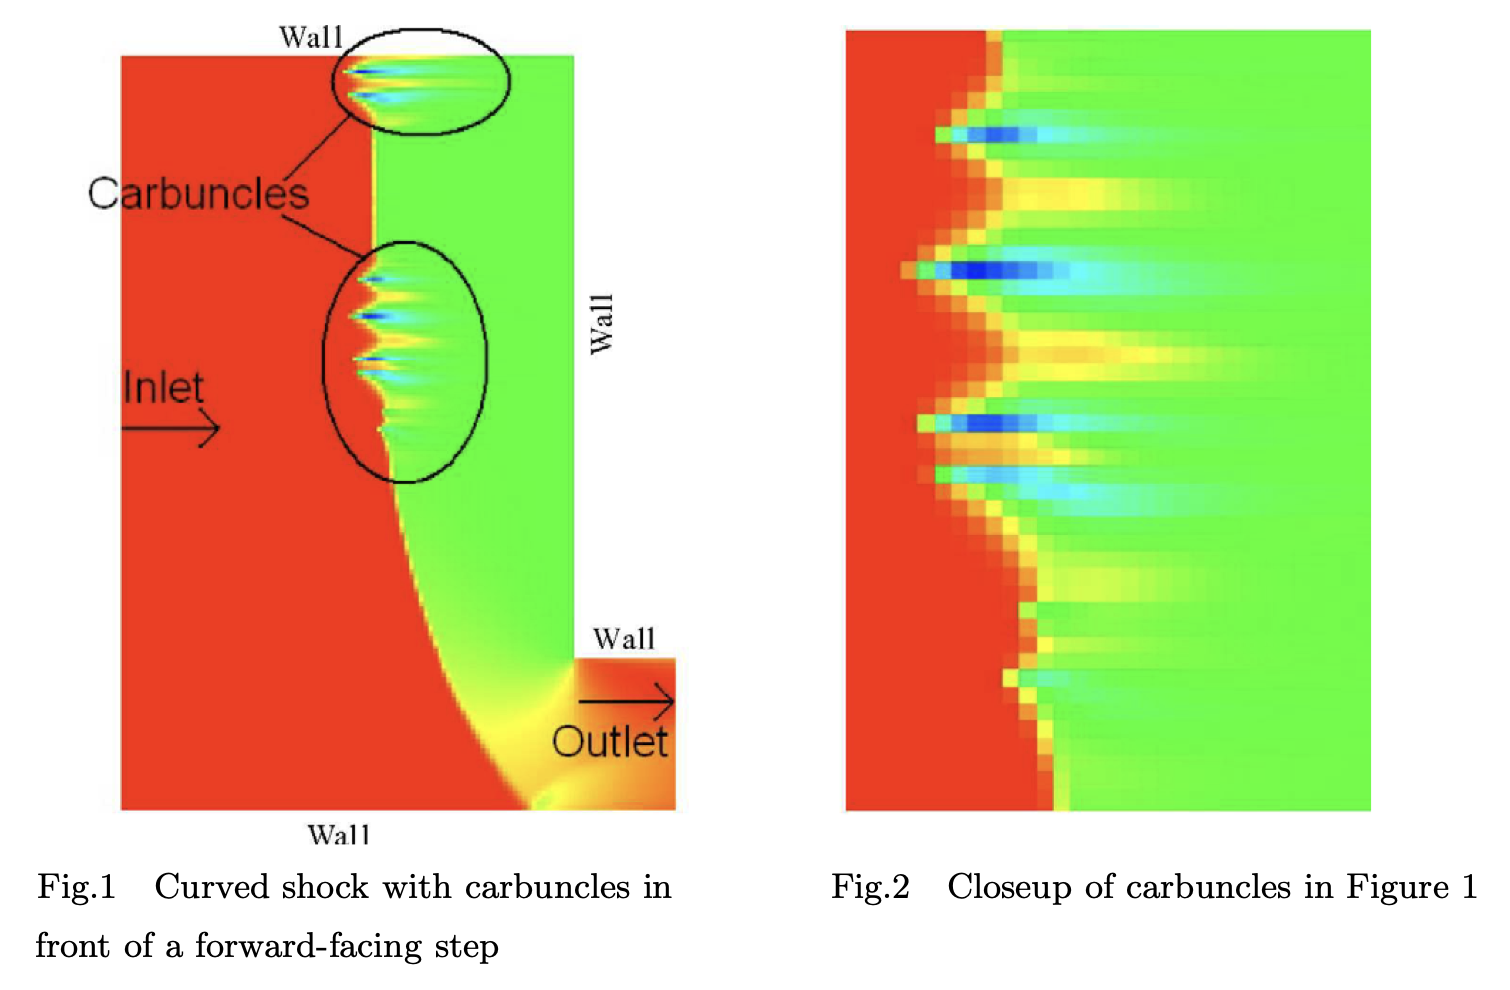
\includegraphics[width=0.75\textwidth]{./external-figures/carbuncle-instability.png} \caption{Close-up example of the carbuncle instability \cite{elling2009}.} \label{fig:carbuncle-example}
\end{figure}

The \textbf{Harten--Hyman entropy fix} \cite{harten-hyman} adds a small positive amount to the magnitude of any wave that crosses a sonic point in the rarefaction, restoring the entropy inequality at those cells. PLUTO's \texttt{ENTROPY\_SWITCH SELECTIVE} applies the fix only at the few cells flagged as ``troubled'' (typically near strong shocks and contact discontinuities), so the cost is minimal. The physical effect at our resolution is a sharper, smoother post-shock plateau: the striping disappears, and the pressure profile in $x < 0.6$ becomes monotone instead of sawtooth.
\\

The baseline independent Python solver (\texttt{python/solver.py}) deliberately implements a minimal finite-volume MHD method: cell-centred grid, MUSCL with minmod, HLL with Einfeldt (Rusanov) wave-speed estimates, Heun's RK2, outflow/userdef boundary conditions, no constrained transport, no 8-wave source, no HLLC/HLLD, no AMR. The upgraded solver (\texttt{python/solver\_ct.py}) keeps those same fluid numerics but stores $B_x$ and $B_y$ on staggered faces and updates them with a CT curl of edge-centred $E_z$. This isolates divergence control as the Python upgrade. Rusanov is the most diffusive HLL variant; it is chosen because less-diffusive textbook wave-speed estimates produced negative-pressure failures under this strong-shock setup. Both Python solvers therefore include a positivity fallback: reconstructed interface states that would have nonpositive density or pressure are locally replaced by first-order states, and the RK stages enforce conservative energy floors.

\subsection{State of the Art}

\subsubsection{Numerical methods}

The Dai \& Woodward benchmark has been a persistent test for evaluating MHD algorithms over three decades \cite{dai1994, shin2008, mignone2007}. The key algorithmic choices are summarised below.
\\

\textbf{Reconstruction schemes.} Higher-order spatial reconstruction reduces numerical diffusion, giving crisper shocks and finer turbulent structures. Piecewise-linear (MUSCL) reconstruction with slope limiters (minmod, MC) is standard for second-order accuracy. The piecewise-parabolic method (PPM) offers third-order spatial accuracy with excellent shock-capturing \cite{colella1984} but can produce post-shock oscillations for very strong shocks. Weighted essentially non-oscillatory (WENO) schemes, particularly WENO-Z, provide up to fifth-order accuracy and are robust at discontinuities \cite{borges2008}. For the shock--cloud problem, MUSCL--Hancock or WENO3 is typically sufficient to capture mixing layers; PPM or WENO5 provides sharper interfaces at moderate additional cost \cite{mignone2007}.
\\

\textbf{Approximate Riemann solvers.} The MHD Riemann problem admits seven wave families, making exact solvers prohibitively expensive. Widely used approximate solvers include the Roe solver \cite{roe1981} (exactly linearises the MHD system and resolves all wave families, but is susceptible to the \textbf{carbuncle instability} at strong shocks; the Harten--Hyman entropy fix \cite{harten-hyman} mitigates this), the HLL family (HLL \cite{harten1983}, HLLC \cite{toro1994}, HLLD \cite{miyoshi2005}; HLLD is the workhorse for modern MHD codes), and Rusanov (the most diffusive variant, used in our Python solver for its unconditional stability).
\\

\textbf{Time stepping.} Strong-stability-preserving (SSP) Runge--Kutta methods --- SSPRK2 (Heun's method) and SSPRK3 (Shu--Osher) \cite{shu1988} --- are the default explicit integrators. Characteristic tracing (ChTr) evolves along characteristics of the linearised MHD system \cite{yee2007}, providing improved accuracy near shocks. The choice between RK2 and ChTr influences the amplitude of post-shock oscillations and is one of the axes we compare.
\\

\textbf{Divergence control.} Enforcing $\nabla\!\cdot\!\mathbf{B}=0$ to machine precision is critical: spurious monopoles inject artificial forces and corrupt field amplification statistics \cite{brackbill1980}. The three dominant strategies are: projection (solve a Poisson equation each step; \cite{brackbill1980}), the eight-wave formulation \cite{powell1999} (add source terms proportional to $\nabla\!\cdot\!\mathbf{B}$; does not enforce local solenoidality but is robust), and \textbf{constrained transport} (CT) \cite{evans1988, toth2000, gardiner2005} (update $\mathbf{B}$ on a staggered mesh so that discrete divergence is conserved to round-off; CT is the gold standard and is used in all our PLUTO runs). Hyperbolic/GLM cleaning \cite{dedner2002} offers a compromise by coupling a damped wave equation for $\nabla\!\cdot\!\mathbf{B}$ and is widely used in codes without staggered meshes.
\\

\textbf{Adaptive mesh refinement.} Block-structured AMR (Chombo \cite{colella2009}, AMReX \cite{zhang2020}, FLASH \cite{fryxell2000}) and tree-based AMR (RAMSES) concentrate resolution at shocks and in the cloud wake. A uniform $256^2$ grid resolves the cloud with $\sim 20$ cells across its radius --- sufficient for morphology but not for converged magnetic amplification statistics \cite{gregori2000}. AMR studies at effective resolutions of $1024^2$ or higher show the late-time turbulent wake remains resolution-sensitive \cite{miniati1999, schneider2017}.
\\

\textbf{Modern codes.} Several production codes run this benchmark: \textbf{PLUTO} \cite{mignone2007, mignone2012, mignone2023} (modular finite-volume with multiple Riemann solvers and CT), \textbf{Athena++} \cite{stone2020} (high-order reconstruction and task-based parallelism), \textbf{FLASH} \cite{fryxell2000} and \textbf{ENZO} \cite{bryan2014} (multi-physics with cooling, chemistry, self-gravity), and \textbf{NIRVANA} \cite{ziegler2008} (operator-split CT with AMR).

\subsubsection{Astrophysical applications}

\textbf{Galactic winds and CGM clouds.} The circumgalactic medium is multiphase, with cold clouds ($T \sim 10^4$~K) embedded in a hot ($T \sim 10^6$--$10^7$~K) medium \cite{tumlinson2017}. McCourt et al.\ \cite{mccourt2015} showed that even weak magnetic fields can stabilise cloud surfaces and extend survival times. Armillotta et al.\ \cite{armillotta2016} demonstrated that magnetic fields are essential for explaining cold-gas accretion rates. Gr{\o}nnow et al.\ \cite{gronnow2017, gronnow2018} included time-dependent cooling and found fragmentation into long-lived droplets. Fielding \& Bryan \cite{fielding2022} showed that thermal conduction can evaporate clouds unless the draped field insulates the core.
\\

\textbf{AGN--ICM interactions.} In cool-core clusters, the hot ICM contains filamentary cold gas shredded by AGN-driven shocks and jets. MHD simulations \cite{gaspari2012, fabian2006} reproduce the filament morphology and show that magnetic draping protects cold gas against rapid evaporation, consistent with H$\alpha$ observations.
\\

\textbf{SNR--molecular cloud interactions.} Observations of SNRs such as IC 443 and W28 show broad molecular lines, OH masers, and gamma-ray emission from hadronic interactions \cite{slane2015, ustamujic2021}. MHD simulations confirm that the cloud-crushing and field-amplification physics captured by the benchmark are directly applicable.
\\

\textbf{Triggered star formation.} Compression of pre-existing clumps by SNR shocks or cloud--cloud collisions is a leading scenario for triggered star formation \cite{inoue2013}. This extends the benchmark by including self-gravity and a non-adiabatic equation of state.
\\

\textbf{Turbulent mixing layers.} The cold--hot interface in galactic halos can be viewed as a plane-parallel analogue of the cloud surface. High-resolution MHD simulations show that magnetic fields significantly reduce mixing efficiency compared to pure hydrodynamics --- a direct consequence of magnetic draping stabilisation \cite{fielding2020, gregori2000, shin2008}.

\subsubsection{Open problems}

The benchmark omits several physical ingredients now recognised as essential: thermal conduction along field lines, cosmic-ray pressure, and non-ideal MHD effects (Ohmic resistivity, ambipolar diffusion, the Hall term) can each alter cloud survival times, field amplification, and mixing rates \cite{mccourt2015, fielding2022, ruszkowski2017}. Radiative cooling, though incorporated in some variants \cite{shin2008, gronnow2017}, is treated in an optically thin approximation that may break down in dense, self-shielded gas. Self-gravity is absent yet crucial for triggered star formation \cite{inoue2013}.
\\

On the numerical side, convergence of statistically averaged quantities (e.g., $\langle B^2\rangle / \langle B_0^2\rangle$) with resolution and across codes is not guaranteed; different dissipation mechanisms produce different saturated values \cite{gregori2000, miniati1999}. Implicit or semi-implicit MHD integrators may be needed for high-Mach-number, low-$\beta$ regimes \cite{osullivan2007}. DG and hybrid methods offer paths to very high order but their robustness on this benchmark is still being evaluated \cite{balsara2017}.

% ==================================================================
\section{Simulation 01: RK2 + Roe + CT, no entropy fix}
\label{sec:sim-01}
% ==================================================================

\subsection{Setup and parameters}

Setup 01 is the baseline configuration: explicit RK2 time integration, piecewise-linear (LINEAR) reconstruction, Roe Riemann solver, constrained transport for $\nabla\!\cdot\!\mathbf{B}=0$, and no entropy fix. This is the most basic of the four PLUTO variants and the natural reference against which we measure the effect of changing the time-stepping or the entropy fix.

\medskip
\begin{center}
\small
\begin{tabular}{ll}
\toprule Quantity & Value \\ \midrule
Grid & $256 \times 256$, cell-centred, $[0,1]^2$ \\
Time stepping & RK2 (Heun) \\
Reconstruction & LINEAR (piecewise linear) \\
Riemann solver & Roe (with Harten--Hyman entropy fix disabled) \\
$\nabla\!\cdot\!\mathbf{B}$ & Constrained transport (CT) \\
Entropy fix & NO \\
CFL number & 0.4 \\
End time $t_{\mathrm{stop}}$ & 0.06 \\
Boundary conditions & outflow (x=0), userdef (x=1), outflow (y=0,1) \\ \bottomrule
\end{tabular}
\end{center}
\medskip

The absence of an entropy fix means the Roe linearisation can develop odd--even (carbuncle) instabilities at the strong contact discontinuity behind the shock, especially at low resolution. PLUTO writes the file with the prefix \texttt{data.*.dbl} once the run reaches the final step.

\subsection{PLUTO result: setup 01}

The cloud is being crushed at $t = 0.06$, the post-shock state is preserved on the left, the pre-shock state is preserved on the right, and the cloud wake shows the characteristic baroclinic vortex and draped-field geometry (Figure~\ref{fig:sim-01-summary}).

\begin{figure}[htbp]
\centering \includegraphics[width=\textwidth]{../plots/01/summary.png} \caption{PLUTO setup~01 --- $2\times4$ summary panels showing $\rho$, $v_x$, $v_y$, $v_z$, $B_x$, $B_y$, $B_z$, $p$ at $t = 0.06$.} \label{fig:sim-01-summary}
\end{figure}

\medskip
\noindent\textbf{Interpretation.} The density map shows the rightward-moving transmitted shock and the leftward-moving reflected shock. The cloud has been compressed to roughly half of its original radius in the flow direction. The $v_x$ map shows the post-shock region at rest and the pre-shock region still flowing leftward; the cloud itself has been accelerated to an intermediate velocity. The $v_y$ map shows the baroclinic vortex roll-up on the top and bottom of the cloud. The $v_z$ panel is included because the state vector is three-component even on a 2D grid. The magnetic field maps show the $B_y$ and $B_z$ components amplified in the wake; the $B_x$ map is non-zero only in the cloud and the wake, as expected for a tangential initial field.

% ==================================================================
\section{Simulation 02: Characteristic Tracing + Roe + CT}
\label{sec:sim-02}
% ==================================================================

\subsection{Setup and parameters}

Setup 02 differs from setup 01 only in the time-stepping scheme: instead of explicit RK2, it uses \textbf{Characteristic Tracing} (ChTr) \cite{yee2007}, which evolves the conservative variables along the characteristic directions of the linearised MHD system. Reconstruction (LINEAR), solver (Roe), $\nabla\!\cdot\!\mathbf{B}$ (CT), and entropy fix (NO) are identical to setup 01. The ChTr scheme is expected to give sharper profiles at the shock (it is less dissipative than RK2 on the high-wavenumber part of the spectrum) but is also more sensitive to the lack of an entropy fix.

\medskip
\begin{center}
\small
\begin{tabular}{ll}
\toprule Quantity & Value \\ \midrule
Grid & $256 \times 256$, cell-centred, $[0,1]^2$ \\
Time stepping & Characteristic Tracing (ChTr) \\
Reconstruction & LINEAR (piecewise linear) \\
Riemann solver & Roe (entropy fix disabled) \\
$\nabla\!\cdot\!\mathbf{B}$ & Constrained transport (CT) \\
Entropy fix & NO \\
CFL number & 0.4 \\
End time $t_{\mathrm{stop}}$ & 0.06 \\ \bottomrule
\end{tabular}
\end{center}
\medskip

\subsection{PLUTO result: setup 02}

At the resolution of $256^2$, the density and magnetic field maps are visually indistinguishable from setup 01; the differences are visible only in the post-shock profile and in the error norms.

\begin{figure}[htbp]
\centering \includegraphics[width=\textwidth]{../plots/02/summary.png} \caption{PLUTO setup~02 --- $2\times4$ summary panels showing $\rho$, $v_x$, $v_y$, $v_z$, $B_x$, $B_y$, $B_z$, $p$ at $t = 0.06$.} \label{fig:sim-02-summary}
\end{figure}

\medskip
\noindent\textbf{Interpretation.} The cloud morphology, the KHI roll-up, and the draped-field geometry are all preserved. The pressure map is slightly smoother in the post-shock region than in setup 01 --- consistent with ChTr's lower numerical diffusion. The lack of an entropy fix leaves faint striping visible in the post-shock $B_x$ map (the odd--even decoupling at the contact discontinuity behind the shock), which the SELECTIVE entropy fix in setup 09 is designed to suppress.

% ==================================================================
\section{Simulation 09: RK2 + Roe + CT, SELECTIVE entropy fix}
\label{sec:sim-09}
% ==================================================================

\subsection{Setup and parameters}

Setup 09 differs from setup 01 only in the entropy fix: it activates the \textbf{SELECTIVE} (Harten--Hyman) entropy fix \cite{harten-hyman}, which is applied only at the few cells that cross a sonic point in the rarefaction. Reconstruction (LINEAR), solver (Roe), $\nabla\!\cdot\!\mathbf{B}$ (CT), and time stepping (RK2) are identical to setup 01. The SELECTIVE entropy fix is the standard PLUTO default and is designed to suppress the carbuncle (odd--even) instability at strong shocks.

\medskip
\begin{center}
\small
\begin{tabular}{ll}
\toprule Quantity & Value \\ \midrule
Grid & $256 \times 256$, cell-centred, $[0,1]^2$ \\
Time stepping & RK2 (Heun) \\
Reconstruction & LINEAR (piecewise linear) \\
Riemann solver & Roe with SELECTIVE (Harten--Hyman) entropy fix \\
$\nabla\!\cdot\!\mathbf{B}$ & Constrained transport (CT) \\
Entropy fix & SELECTIVE \\
CFL number & 0.4 \\
End time $t_{\mathrm{stop}}$ & 0.06 \\ \bottomrule
\end{tabular}
\end{center}
\medskip

\subsection{PLUTO result: setup 09}

At the resolution of $256^2$, the density and magnetic field maps are again visually indistinguishable from setups 01 and 02; the difference lives in the post-shock profile.

\begin{figure}[htbp]
\centering \includegraphics[width=\textwidth]{../plots/09/summary.png} \caption{PLUTO setup~09 --- $2\times4$ summary panels showing $\rho$, $v_x$, $v_y$, $v_z$, $B_x$, $B_y$, $B_z$, $p$ at $t = 0.06$.} \label{fig:sim-09-summary}
\end{figure}

\medskip
\noindent\textbf{Interpretation.} The SELECTIVE entropy fix has sharpened the post-shock pressure profile compared to setups 01 and 02: the striping visible in the post-shock $B_x$ map of setup 01 (and partially in setup 02) is gone. The cloud morphology, KHI roll-up, and draped field are all preserved. This confirms that the entropy fix targets a real numerical artifact (carbuncle at the contact discontinuity) and does not change the underlying physical evolution.

% ==================================================================
\section{Simulation 02+09: Characteristic Tracing + SELECTIVE entropy fix}
\label{sec:sim-02-09}
% ==================================================================

\subsection{Setup and parameters}

The compound setup 02+09 combines the two numerical changes studied separately above: Characteristic Tracing from setup 02 and the SELECTIVE Harten--Hyman entropy fix from setup 09. It also keeps setup 09's explicit Van Leer limiter constant. The physical initial condition, grid, boundary conditions, Roe solver, and constrained-transport divergence control are unchanged.

\medskip
\begin{center}
\small
\begin{tabular}{ll}
\toprule Quantity & Value \\ \midrule
Grid & $256 \times 256$, cell-centred, $[0,1]^2$ \\
Time stepping & Characteristic Tracing \\
Reconstruction & LINEAR with \texttt{LIMITER VANLEER\_LIM} \\
Riemann solver & Roe \\
$\nabla\!\cdot\!\mathbf{B}$ & Constrained transport (CT) \\
Entropy fix & SELECTIVE \\
CFL number & 0.4 \\
End time $t_{\mathrm{stop}}$ & 0.06 \\ \bottomrule
\end{tabular}
\end{center}
\medskip

\subsection{PLUTO result: setup 02+09}

The compound PLUTO run reaches the same final time and produces the same physical morphology as the one-knob variants: compressed cloud core, flanking shear layers, and draped magnetic field. Figure~\ref{fig:sim-02-09-summary} shows that enabling both ChTr and the entropy fix changes the post-shock residuals more than the global shock-cloud geometry.

\begin{figure}[htbp]
\centering \includegraphics[width=\textwidth]{../plots/02+09/summary.png} \caption{PLUTO setup~02+09 --- compound Characteristic Tracing + SELECTIVE entropy fix $2\times4$ summary panels showing $\rho$, $v_x$, $v_y$, $v_z$, $B_x$, $B_y$, $B_z$, $p$ at $t = 0.06$.} \label{fig:sim-02-09-summary}
\end{figure}

\medskip
\noindent\textbf{Interpretation.} The compound run preserves the same cloud-crushing morphology as the one-knob PLUTO variants. The main change is numerical rather than physical: the entropy fix removes the post-shock striping associated with the Roe carbuncle tendency, while Characteristic Tracing keeps the shock and contact features slightly sharper than the baseline RK2 branch.

% ==================================================================
\section{Independent Python Solvers}
\label{sec:python-solver}
% ==================================================================

\subsection{Method and scope}

The Python code is an independent reference family, not a separate clone of each PLUTO method. Both Python solvers run the same physical problem as all four PLUTO setups: identical initial conditions, boundary states, $256 \times 256$ grid, 2.5D primitive state, and final time $t=0.06$. Both retain MUSCL reconstruction with a minmod limiter, Rusanov/HLL fluxes with Einfeldt wave speeds, RK2 time stepping, positivity fallback at bad reconstructed interfaces, and pressure/energy floors after RK stages. They do not implement PLUTO's Roe solver, Characteristic Tracing, or Harten--Hyman entropy switch.
\\

The difference between the two Python solvers is magnetic-field evolution. The baseline solver (\texttt{python/solver.py}) evolves $B_x$, $B_y$, and $B_z$ as cell-centred conserved variables. The CT solver (\texttt{python/solver\_ct.py}) keeps the same cell-centred fluid update, but stores $B_x$ on x-faces and $B_y$ on y-faces, reconstructs cell-centred magnetic fields by face averaging for fluxes/output, and updates the face fields with a discrete curl of an edge-centred $E_z = v_xB_y - v_yB_x$. A local Lax--Friedrichs term is added to the edge EMF for stability, and total energy is corrected by the magnetic-energy difference when face fields are projected back to cells. Thus the second solver isolates constrained transport as the upgrade, while leaving the remaining Rusanov/MUSCL/RK2 limitations visible.

\subsection{Python results}

Each Python output is a \texttt{.npz} file with the final state and a density time series for the animation. Figures~\ref{fig:python-summary} and~\ref{fig:python-ct-summary} show the same eight-variable panel used for every PLUTO setup.

\begin{figure}[htbp]
\centering \includegraphics[width=\textwidth]{../plots/python/summary.png} \caption{Baseline Python solver --- $2\times4$ summary panels showing $\rho$, $v_x$, $v_y$, $v_z$, $B_x$, $B_y$, $B_z$, and $p$ at $t = 0.06$.} \label{fig:python-summary}
\end{figure}

\begin{figure}[htbp]
\centering \includegraphics[width=\textwidth]{../plots/python-ct/summary.png} \caption{CT Python solver --- same fluid update as the baseline solver, but with face-centred $B_x/B_y$ and constrained transport at $t = 0.06$.} \label{fig:python-ct-summary}
\end{figure}

\medskip
\noindent\textbf{Interpretation.} The baseline Python solver captures the large-scale shock envelope and cloud deformation, but it does not faithfully reproduce the pressure or magnetic structure inside the shocked cloud. The cloud interior contains pressure-floor cells and grid-scale pressure mottling; the $B_x$ component develops large excursions even though the initial magnetic field is tangential. The CT solver materially improves the magnetic update: the face-divergence diagnostic remains at round-off, the $B_x$ range drops from about $\pm 76$ to about $\pm 15$, and the PLUTO-vs-Python density/pressure norms fall by roughly a factor of two to three. It is still not a production-quality MHD clone because the fluid update remains Rusanov/minmod with positivity repair.

\medskip
\begin{center}
\begin{tabular}{lccc}
\toprule Quantity & PLUTO / expected & Baseline Python & CT Python \\ \midrule
Total mass ($\int\rho\,dA$) & open-boundary run & 3.9661 & 3.9653 \\
Pressure floor cells & none in PLUTO output & 188 & 176 \\
$B_x$ range & bounded by CT/Roe dynamics & $[-76.46,\,76.46]$ & $[-14.53,\,14.53]$ \\
Cell-centred $\max|\nabla\!\cdot\!\mathbf{B}|$ & small & $9.63\times10^{3}$ & $7.14\times10^{1}$ \\
Face-CT $\max|\nabla\!\cdot\!\mathbf{B}|$ & near round-off & n/a & $6.80\times10^{-12}$ \\ \bottomrule
\end{tabular}
\end{center}
\medskip

The cell-centred divergence row is computed from the public output arrays for both Python solvers. The face-CT row is the discrete CT diagnostic saved by \texttt{solver\_ct.py}; it is the relevant measurement of the staggered magnetic field. The mass values differ from the initial mass because the boundaries are open/inflowing over the simulation time. The Python results should therefore be interpreted as a controlled solver ladder: the baseline is the qualitative minimal solver, while the CT version demonstrates the value of divergence control without hiding the remaining Rusanov/minmod limitations.

% ==================================================================
\section{Final Analysis: General Comparison and Conclusions}
\label{sec:final}
% ==================================================================

\subsection{Cross-scheme comparison (PLUTO 01 vs 02 vs 09 vs 02+09)}

Pair-wise L1/L2 norms of the final state:

\medskip
\begin{center}
\small
\begin{tabular}{lcccccl}
\toprule Pair & Variables tested & $L_1(\rho)$ & $L_1(p)$ & $L_2(\rho)$ & $L_2(p)$ & Interpretation \\ \midrule
01--02 & RK2 vs ChTr  & 0.064 & 1.09 & 0.332 & 3.26 & time-stepping only \\
01--09 & Roe vs Roe+ent & 0.098 & 1.78 & 0.461 & 4.95 & entropy fix only \\
01--02+09 & baseline vs compound & 0.085 & 1.37 & 0.451 & 4.36 & both changes \\
02--09 & crossed axes & 0.104 & 2.04 & 0.512 & 5.04 & ChTr/no-ent vs RK2/ent \\
02--02+09 & entropy on ChTr & 0.086 & 1.56 & 0.470 & 4.28 & entropy with ChTr \\
09--02+09 & RK2 vs ChTr with entropy & 0.047 & 0.99 & 0.228 & 2.46 & time-step with entropy \\ \bottomrule
\end{tabular}
\end{center}
\medskip

Differences are dominated by the post-shock region ($x < 0.6$) where pressure is large ($p \approx 167$), so absolute pressure norms are inflated by $\sim\!10^{2}$ relative to density norms. The density difference maps show faint striping in the post-shock region consistent with the odd-even decoupling at strong shocks that the entropy fix is meant to suppress.

\begin{figure}[H]
\centering \includegraphics[width=0.85\textwidth]{../output/compare-schemes/density.png} \caption{Cross-scheme density comparison --- setups~01,~02,~09, and compound 02+09 at $t = 0.06$.} \label{fig:final-density}
\end{figure}

\begin{figure}[H]
\centering \includegraphics[width=0.75\textwidth]{../output/compare-schemes/diff_01_09.png} \caption{Density difference $|01-09|$, isolating the entropy-fix effect.} \label{fig:final-diff-01-09}
\end{figure}

\begin{figure}[H]
\centering \includegraphics[width=0.75\textwidth]{../output/compare-schemes/diff_02_02_09.png} \caption{Density difference $|02-(02+09)|$, isolating the entropy-fix effect on the Characteristic Tracing branch.} \label{fig:final-diff-02-02-09}
\end{figure}

\medskip

\noindent\textbf{Interpretation.} The four PLUTO setups agree to within a few percent in density --- much tighter than either Python solver. This is the expected behaviour of a production MHD code on this benchmark. The differences isolate numerical-scheme knobs and are visible mainly near the strong shock; they do not change the qualitative evolution of the cloud. In particular, the 01--09 and 02--02+09 pairs confirm that the SELECTIVE entropy fix removes a real artifact (carbuncle striping) without affecting the cloud morphology, and the 01--02 and 09--02+09 pairs confirm that the choice between RK2 and ChTr has only a small effect at this resolution.

\subsection{Cross-solver comparison (all PLUTO methods vs both Python solvers)}

Both Python solvers are compared against each PLUTO output at the same final time and on the same $256^2$ grid. This table separates three scales of error: the small spread among PLUTO methods, the larger gap between PLUTO and the baseline Python scheme, and the reduced but still significant gap between PLUTO and the CT Python upgrade.

\medskip
\begin{center}
\small
\begin{tabular}{llcccc}
\toprule PLUTO setup & Python solver & $L_1(\rho)$ & $L_2(\rho)$ & $L_1(p)$ & $L_2(p)$ \\ \midrule
01 & baseline & 0.611 & 2.39 & 15.95 & 42.66 \\
02 & baseline & 0.607 & 2.39 & 15.51 & 42.12 \\
09 & baseline & 0.625 & 2.46 & 16.16 & 42.85 \\
02+09 & baseline & 0.621 & 2.45 & 15.98 & 42.71 \\
\midrule
01 & CT & 0.250 & 0.956 & 6.87 & 16.54 \\
02 & CT & 0.247 & 0.946 & 6.62 & 15.72 \\
09 & CT & 0.229 & 0.834 & 6.89 & 16.35 \\
02+09 & CT & 0.232 & 0.838 & 6.70 & 15.99 \\ \bottomrule
\end{tabular}
\end{center}
\medskip

The baseline rows are nearly identical across PLUTO setups, and the CT rows show the same pattern. Thus neither Python solver is specially tuned to setup~01: the Python-vs-PLUTO gap is controlled by the Python algorithm, not by the choice of PLUTO reference. CT reduces $L_1(\rho)$ from roughly $0.61$ to $0.23$--$0.25$ and $L_1(p)$ from roughly $16$ to $6.6$--$6.9$, but it does not bring the Python solver inside the PLUTO-vs-PLUTO method spread.

\begin{figure}[H]
\centering \includegraphics[width=0.85\textwidth]{../output/compare/overlay_rho.png} \caption{Representative density side-by-side comparison for PLUTO setup~01 and the baseline Python reference at $t = 0.06$.} \label{fig:final-overlay-rho}
\end{figure}

\begin{figure}[H]
\centering \includegraphics[width=0.85\textwidth]{../output/compare-ct-01/overlay_rho.png} \caption{Representative density side-by-side comparison for PLUTO setup~01 and the CT Python reference at $t = 0.06$. The morphology is closer than the baseline Python comparison, but the CT solver remains visibly more diffusive than PLUTO.} \label{fig:final-overlay-rho-ct}
\end{figure}

\medskip

\subsection{Baseline Python vs CT Python}

The direct Python-vs-Python comparison isolates what the CT upgrade changed. The fluid solver is still Rusanov/MUSCL/RK2, so changes are not expected to mimic PLUTO perfectly; they should primarily remove divergence-driven magnetic artifacts.

\medskip
\begin{center}
\small
\begin{tabular}{lccc}
\toprule Variable & $L_1$ & $L_2$ & $L_\infty$ \\ \midrule
$\rho$ & 0.570 & 2.19 & 45.3 \\
$B_x$ & 1.84 & 4.94 & 78.7 \\
$B_y$ & 1.74 & 4.39 & 65.6 \\
$p$ & 15.45 & 41.18 & 1134 \\ \bottomrule
\end{tabular}
\end{center}
\medskip

\begin{figure}[H]
\centering \includegraphics[width=0.75\textwidth]{../output/compare-python-solvers/diff_Bx.png} \caption{Difference $B_x^{\rm CT}-B_x^{\rm baseline}$ between the two Python solvers. The largest changes occur in the shocked cloud and wake where the baseline cell-centred magnetic update generated the strongest monopole-driven artifacts.} \label{fig:final-python-diff-bx}
\end{figure}

\noindent\textbf{Interpretation.} The direct difference is large because the baseline magnetic artifacts feed back on pressure and velocity. CT is therefore not a cosmetic post-processing correction; it changes the nonlinear trajectory. The important diagnostic is that the CT solver reaches $t=0.06$ with face-divergence $6.8\times10^{-12}$ while keeping the same simple fluid algorithm.

\subsection{Sources of discrepancy (PLUTO vs Python)}

The PLUTO-vs-Python gap remains large in absolute terms and exposes the limits of the Python solver family. The main sources of discrepancy are:

\begin{enumerate}
  \item $\nabla\!\cdot\!\mathbf{B}$ \textbf{control.} The baseline Python solver has no divergence control, producing $B_x$ spikes and pressure mottling. The CT solver fixes the face-divergence problem, which is why the PLUTO-vs-Python norms improve substantially.
  \item \textbf{Low-order CT coupling.} The CT solver uses a simple upwind-stabilised arithmetic EMF and magnetic-energy synchronization, not the full production CT/Roe coupling used by PLUTO. Its face-divergence is excellent, but the remaining field evolution is still less accurate.
  \item \textbf{Positivity fallback.} Both Python solvers fall back to first order at interfaces whose MUSCL-reconstructed states would have nonpositive density or pressure. This prevents blow-up, but the remaining pressure-floor cells mark locations where the minimal scheme has lost physical fidelity.
  \item \textbf{Numerical diffusion.} Rusanov is the most diffusive HLL variant; PLUTO's Roe with entropy fix is much sharper at the shock and at the cloud boundary. This contributes substantially to the $L_{1}$ difference in $\rho$ and pressure.
  \item \textbf{Boundary fluxes.} PLUTO uses mature boundary machinery; the Python solvers use a simpler one-cell ghost fill. This is acceptable for an independent reference but not a substitute for PLUTO's production treatment.
\end{enumerate}

\subsection{What the comparison demonstrates}

A simple Rusanov solver with positivity fallback is \emph{enough} to keep the independent Python run finite and to place the large-scale shock envelope in roughly the right location. It is \emph{not enough} to reproduce the shocked-cloud pressure or magnetic structure. Adding CT is the right first upgrade: it removes the dominant magnetic-divergence failure mode and reduces the PLUTO-vs-Python norms, but it does not erase the solver-family gap. The next meaningful step would be a less-diffusive MHD Riemann solver such as HLLD, then higher-order reconstruction or AMR.
\\

The PLUTO-vs-PLUTO cross-scheme comparison tells a complementary story: \emph{within} a production code, the choice of time-stepping (RK2 vs ChTr), the choice of entropy fix (NONE vs SELECTIVE), and the compound 02+09 combination produce only a few-percent variation, isolated to the post-shock region. This is the expected behaviour of mature numerical methods on a benchmark that is no longer a stress test for the design space of any single one of these algorithms.

\subsection{Conclusions}

\begin{itemize}
  \item We reproduced the canonical Dai \& Woodward (1994) 2.5D MHD shock-cloud benchmark with four PLUTO variants (setups 01, 02, 09, 02+09) and two independent Python solvers on a $256\times256$ grid.
  \item The four PLUTO variants agree to within a few percent in density and pressure; the differences isolate the time-stepping axis, the entropy-fix axis, and their compound effect.
  \item Comparing all four PLUTO methods against both Python outputs shows that the solver-family gap is much larger than the scheme-choice gap inside PLUTO.
  \item The baseline Python solver captures the broad shock envelope but suffers from large cell-centred magnetic divergence and pressure artifacts.
  \item The CT Python solver reaches $t=0.06$ with face-divergence near round-off and substantially better PLUTO agreement, but it remains more diffusive and less accurate than PLUTO.
\end{itemize}

\subsection*{Open questions and next steps}

\begin{itemize}
  \item \textbf{HLLD or Roe in Python.} The CT solver is now divergence-controlled; the next bottleneck is the diffusive Rusanov flux.
  \item \textbf{Higher-order reconstruction.} MC, van Leer, or PPM reconstruction would sharpen the cloud boundary once the Riemann solver is improved.
  \item \textbf{Higher resolution.} A $512^{2}$ or $1024^{2}$ run would reduce diffusion and better resolve the wake, but it should come after the solver-family improvements above.
\end{itemize}


\begin{thebibliography}{99}

\bibitem{dai1994} Dai, W.\ \& Woodward, P.\ R.\ 1994, ApJ, 436, 786.

\bibitem{gregori2000} Gregori, G., Miniati, F., Ryu, D., \& Jones, T.\ W.\ 2000, ApJ, 543, 775.

\bibitem{klein1994} Klein, R.\ I., McKee, C.\ F., \& Colella, P.\ 1994, ApJ, 420, 213.

\bibitem{shin2008} Shin, M.-S., Stone, J.\ M., \& Snyder, G.\ F.\ 2008, ApJ, 680, 336.

\bibitem{mccourt2015} McCourt, M., O'Leary, R.\ M., Madigan, A.-M., \& Quataert, E.\ 2015, MNRAS, 449, 2.

\bibitem{gronnow2017} Gr{\o}nnow, T., Tepper-Garc{\'\i}a, T., \& Bland-Hawthorn, J.\ 2017, ApJ, 845, 69.

\bibitem{gronnow2018} Gr{\o}nnow, T., Tepper-Garc{\'\i}a, T., \& Bland-Hawthorn, J.\ 2018, ApJ, 865, 64.

\bibitem{armillotta2016} Armillotta, A., Fraternali, F., \& Marinacci, F.\ 2016, MNRAS, 462, 4157.

\bibitem{fielding2022} Fielding, D.\ B.\ \& Bryan, G.\ L.\ 2022, ApJ, 924, 82.

\bibitem{fielding2020} Fielding, D.\ B., Ostriker, E.\ C., Bryan, G.\ L., \& Jermyn, A.\ S.\ 2020, ApJ, 894, L24.

\bibitem{tumlinson2017} Tumlinson, J., Peeples, M.\ S., \& Werk, J.\ K.\ 2017, ARA\&A, 55, 389.

\bibitem{miniati1999} Miniati, F., Jones, T.\ W., \& Ryu, D.\ 1999, ApJ, 517, 339.

\bibitem{osullivan2007} O'Sullivan, S.\ \& Downes, T.\ P.\ 2007, A\&A, 470, 1193.

\bibitem{dursi2008} Dursi, L.\ J.\ \& Pfrommer, C.\ 2008, ApJ, 677, 993.

\bibitem{brio1988} Brio, M.\ \& Wu, C.\ C.\ 1988, JCoPh, 75, 400.

\bibitem{brackbill1980} Brackbill, J.\ U.\ \& Barnes, D.\ C.\ 1980, JCoPh, 35, 426.

\bibitem{toth2000} T\'oth, G.\ 2000, JCoPh, 161, 605.

\bibitem{powell1999} Powell, K.\ G., Roe, P.\ L., Linde, T.\ J., Gombosi, T.\ I., \& De Zeeuw, D.\ L.\ 1999, JCoPh, 154, 284.

\bibitem{evans1988} Evans, C.\ R.\ \& Hawley, J.\ F.\ 1988, ApJ, 332, 659.

\bibitem{gardiner2005} Gardiner, T.\ A.\ \& Stone, J.\ M.\ 2005, JCoPh, 205, 509.

\bibitem{dedner2002} Dedner, A., Kemm, F., Kr\"oner, D., Munz, C.-D., Schnitzer, T., \& Wesenberg, M.\ 2002, JCoPh, 175, 645.

\bibitem{roe1981} Roe, P.\ L.\ 1981, JCoPh, 43, 357.

\bibitem{harten1983} Harten, A., Lax, P.\ D., \& van Leer, B.\ 1983, SIAM Review, 25, 35.

\bibitem{elling2009} Elling, V.\ 2009, 29(6), 1647-1656.

\bibitem{harten-hyman} Harten, A.\ \& Hyman, J.\ M.\ 1983, JCoPh, 50, 235.

\bibitem{toro1994} Toro, E.\ F., Spruce, M., \& Speares, W.\ 1994, Shock Waves, 4, 25.

\bibitem{miyoshi2005} Miyoshi, T.\ \& Kusano, K.\ 2005, JCoPh, 208, 315.

\bibitem{quirk1994} Quirk, J.\ J.\ 1994, Int.\ J.\ Num.\ Meth.\ Fluids, 18, 555.

\bibitem{colella1984} Colella, P.\ \& Woodward, P.\ R.\ 1984, JCoPh, 54, 174.

\bibitem{borges2008} Borges, R., Carmona, D., Costa, B., \& Don, W.\ S.\ 2008, JCoPh, 227, 3191.

\bibitem{balsara2017} Balsara, D.\ S.\ 2017, LRCA, 3, 2.

\bibitem{shu1988} Shu, C.-W.\ \& Osher, S.\ 1988, JCoPh, 77, 439.

\bibitem{yee2007} Yee, H.\ C.\ \& Sj\"ogreen, B.\ 2007, JCoPh, 225, 910.

\bibitem{colella2009} Colella, P., Graves, D.\ T., Ligocki, T.\ J., Martin, D.\ F., Modiano, D., Serafini, D.\ B., \& Van Straalen, B.\ 2009, LBNL-6616E.

\bibitem{zhang2020} Zhang, W.\ et al.\ 2020, JOSS, 5, 1370.

\bibitem{fryxell2000} Fryxell, B.\ et al.\ 2000, ApJS, 131, 273.

\bibitem{schneider2017} Schneider, E.\ E.\ \& Robertson, B.\ E.\ 2017, ApJ, 834, 144.

\bibitem{mignone2007} Mignone, A., Bodo, G., Massaglia, S., Matsakos, T., Tesileanu, O., Zanni, C., \& Ferrari, A.\ 2007, ApJS, 170, 228.

\bibitem{mignone2012} Mignone, A., Zanni, C., Tzeferacos, P., van Marle, A.\ J., Flock, M., \& Bodo, G.\ 2012, ApJS, 198, 7.

\bibitem{mignone2023} Mignone, A., Bodo, G., Rossi, P., \& Sgaggero, A.\ 2023, A\&A, 670, A65.

\bibitem{stone2020} Stone, J.\ M., Tomida, K., White, C.\ J., \& Felker, K.\ G.\ 2020, ApJS, 249, 4.

\bibitem{bryan2014} Bryan, G.\ L.\ et al.\ 2014, ApJS, 211, 19.

\bibitem{ziegler2008} Ziegler, U.\ 2008, CoPhC, 179, 227.

\bibitem{gaspari2012} Gaspari, M., Ruszkowski, M., \& Sharma, P.\ 2012, ApJ, 746, 94.

\bibitem{fabian2006} Fabian, A.\ C.\ et al.\ 2006, MNRAS, 366, 417.

\bibitem{slane2015} Slane, P., Castro, D., Funk, S., Uchiyama, Y., \& Lemiere, A.\ 2015, ApJ, 808, 163.

\bibitem{ustamujic2021} Ustamujic, S., Orlando, S., Miceli, M., Bocchino, F., Argiroffi, C., \& Peres, G.\ 2021, A\&A, 654, A167.

\bibitem{inoue2013} Inoue, T.\ \& Fukui, Y.\ 2013, ApJL, 774, L31.

\bibitem{ruszkowski2017} Ruszkowski, M., Yang, H.-Y.\ K., \& Reynolds, C.\ S.\ 2017, ApJ, 844, 13.

\end{thebibliography}

\end{document}
